\documentclass[a4paper]{article}
\usepackage[ngerman]{babel}
\usepackage{amsthm}
\usepackage{amsmath}
\usepackage{amsfonts}
\usepackage{parskip}
\usepackage{graphicx}
\usepackage{color}
\usepackage{listings}

\usepackage{color}

\definecolor{mygreen}{rgb}{0,0.6,0}
\definecolor{mygray}{rgb}{0.5,0.5,0.5}
\definecolor{mymauve}{rgb}{0.58,0,0.82}

\lstset{ 
  backgroundcolor=\color{white},
  basicstyle=\footnotesize,
  breakatwhitespace=false,
  breaklines=true,
  captionpos=b,
  commentstyle=\color{mygreen},
  extendedchars=true,
  frame=single,
  keepspaces=true,
  keywordstyle=\color{blue},
  language=Java,
  numbers=left,
  numbersep=5pt,
  numberstyle=\color{mygray},
  rulecolor=\color{black},
  showspaces=false,
  showstringspaces=false,
  showtabs=false,
  stepnumber=5,
  stringstyle=\color{mymauve},
  tabsize=2,
  title=\lstname
}

\pagestyle{headings}

\newtheorem{satz}{Satz}
\theoremstyle{definition}
\newtheorem{definition}{Definition}

\title{Dokumentation}
\author{
    Matthias Vonend
    \and
    Jan Grübener
    \and
    Patrick Mischka
    \and
    Michael Angermeier
    \and
    Troy Keßler
    \and
    Aaron Schweig
    \and
}

\begin{document}

    \maketitle
    \tableofcontents

    % oder clearpage
    \vspace{0.2cm}

    % TODO add information about git

    \section{Basisanforderungen}
        % !TEX root = ./docs.tex




\begin{figure}[h]
    \centering
    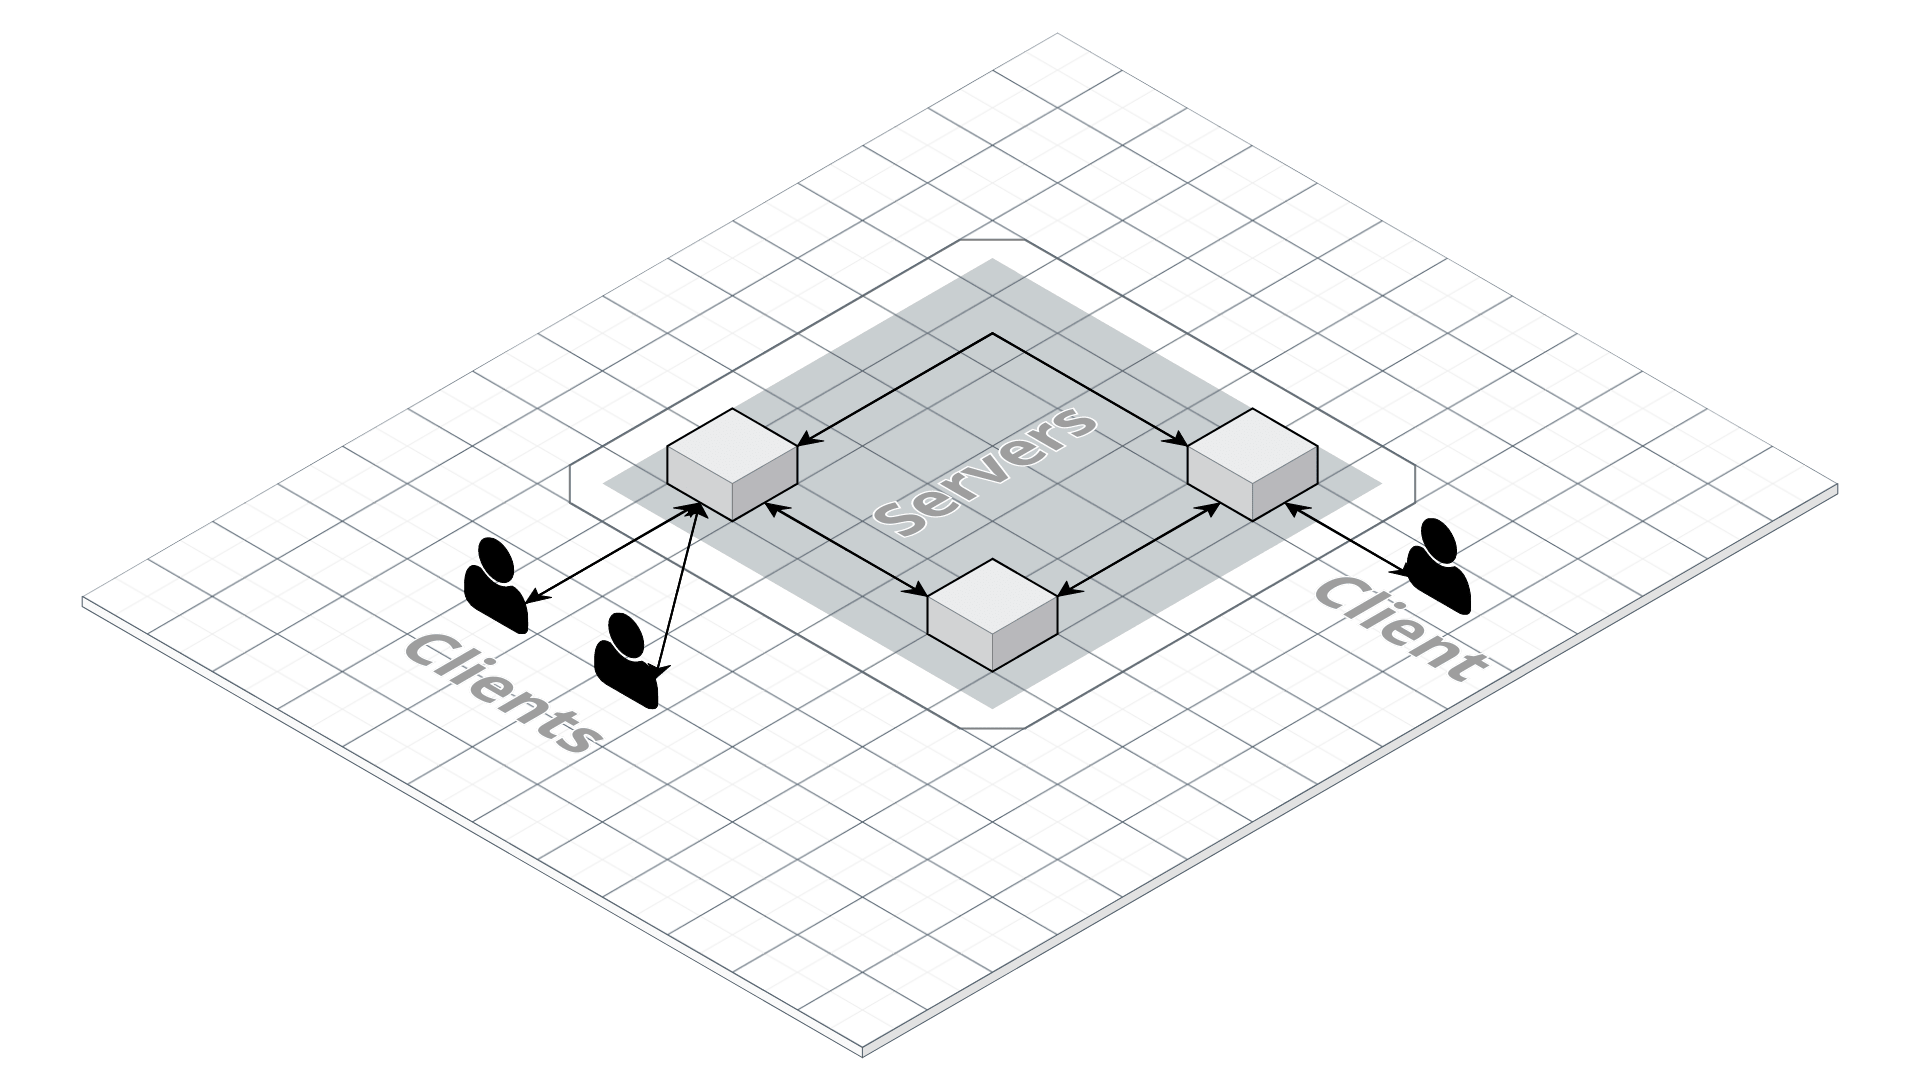
\includegraphics[width=\textwidth]{architecture.png}
    
    \caption{Architektur}
    \label{}
\end{figure}

\subsection{Chatfunktionalität}
Damit ein Chat ablaufen kann muss zunächst eine Verbindung zu einem Server aufgebaut werden. Dazu wählt der Client zunächst einen zufälligen Server aus und versucht sich zu verbinden. Wurde eine Verbindung erfolgreich aufgebaut, kann sich der Nutzer mit seinem Nutzername und seinem Password anmelden. Sobald der Nutzer angemeldet ist sendet der Server ihm alle benötigten Informationen inklusiver der verpassten Nachrichten. Jede Nachricht hat eine Datum wann es erstmalig an einem Server eingetroffen ist. Anhand von diesem werden die Nachrichten sortiert, damit der Client die korrekte Reihenfolge darstellen kann.

Möchte dieser eine Nachricht an einen weiteren Client senden, schickt er diese an seine verbundene Node und überlässt die Zustellung dieser. Da alle Nachrichten aus Persistenzgründen an alle Nodes verteilt werden müssen, brauchen die Nodes keine Information über die Clients anderer Nodes. Im Falle einer solchen Anforderung (z.\,B. Abfrage ob ein anderer Nutzer aktiv ist) könnte ein Protokoll ähnlich zu Routing-Tabellen implementiert werden. Empfängt eine Node eine Nachricht, egal ob von einem Client oder von einer anderen Node, überprüft diese ob die Nachricht für einen ihr bekannten Client bestimmt war und sendet diese gegebenenfalls an diesen.

//TODO Nach einer erfolgreichen Anmeldung kann der Nutzer
// create chat und so bla :)


\subsection{Fehlerbehandlung}
Aus den Anforderungen geht hervor, dass es mindestens zwei Server geben muss, die sämtliche Informationen des Chatsystems besitzen müssen. Bricht eine Node zusammen muss dementsprechend eine andere Node dessen Aufgabe übernehmen.
\subsubsection{Client}
//TODO Troy

Im Fehlerfall scheitert das Senden einer Nachricht an den Server. In diesem Fall versucht sich der Client mit einer anderen Node zu verbinden und sendet die Nachricht erneut.

\subsubsection{Server}
Serverseitig können verschiedene Fehler auftretten. VIele Fehler werden bereits durch das TCP-Protokoll verhindert. Dennoch können grundsätzlich die folgende Fehlerfälle eintretten:
\begin{enumerate}
    \item Nachricht des Clients kann nicht korrekt empfangen/gesendet werden\\
        In diesem Fall muss der Server davon ausgehen, dass die Verbindung zusammengebrochen ist und er beendet seine Verbindung. Der Server verlässt sich darauf, dass der Client erneut eine Verbindung aufbaut. Alle für den Client relevanten Nachrichten werden dann zu diesem übertragen und der Client muss neue Informationen zurück übertragen
    \item Nachrichten einer Nachbarnode können nicht korrekt empfangen/gesendet werden\\
        Ähnlich zur Clientverbindung muss der Server davon ausgehen dass die Verbindung zusammengebrochen ist. Allerdings ist der Server hier selbst dafür zuständig sich erneut zu verbinden. Sämtliche Nachrichten, die an eine Node gesendet werden müssen werden in einer Queue aufbewahrt und nacheinander gesendet. Scheitert die Verbindung, so bleibt die Queue unverändert und wird nach einem erneuten Verbinden weiter abgearbeitet. Es wird solange versucht zu verbinden, bis eine Verbindung zustande gekommen ist. Sobald eine Verbindung wieder aufgebaut wurde synchronisieren sich die Nodes um wieder einen vollständigen Informationsstand zu besitzen.
        Sind keine Nachrichten zu senden hat die Node keine Möglichkeit festzustellen ob eine Verbindung noch existiert. Zu diesem Zweck existiert ein Heartbeat, der periodisch die Nachbarnodes anpingt und so prüft ob die Verbindung noch existiert.
\end{enumerate}
Wie gerade beschrieben führen alle beteiligten stehts eine synchronisation durch wodurch diese immer den kompletten Informationsbestand besitzen.

Eine Veränderung des Datenbestandes muss dem entsprechend an alle anderen Nodes weiter gegeben werden. Dadurch sind alle Server gleichwertige Servern.





    \section{Erweiterungen}
        % !TEX root = ./docs.tex

\subsection{Grafische Oberfläche bei den Nutzern}

\subsection{Verwendung von Emojis}

\subsection{Mehrere Chatverläufe pro Nutzer}

\subsection{Persistentes Speichern der Chatverläufe}

\subsection{Verschlüsselte serverseitige Speicherung der Chats}

\subsection{Gruppenchats}

\subsection{Verschlüsselte Übertragung der Chat-Nachrichten}

%\subsection{3 replizierte Server mit Majority Consensus Strategie}
% Gibt in unserem Ansatz keinen Sinn


    \clearpage
    \section{Anhang}
        % !TEX root = ./docs.tex



\lstinputlisting[linerange={37-76}, firstnumber=37]{../src/main/java/vs/chat/server/ConnectionHandler.java}
 % Per section? -> problematic ref


    \section{TODOS}
        Das doc schreiben duh :P
        Konfliktvermeidung ansprechen -> Datenbanken vergleich mit UUID als Fremdschlüssel
        UUIDs erwähnen
        Code walkthrough + kommentieren
        Titlepage überarbeiten



    \section{TEMP Codewalkthrough}
    Entrypoint ist der Serverbootstrapper. Dieser erstellt einen neuen Thread mit einem neuen Server. Der Server erstellt die Listener, die die zu empfangenen Packete handeln werden. Anschließend werden die Filter erstellt, die bestimmen, ob ein Packet gehandelt oder ignoriert werden soll (z.B. bei recursiven Broadcasts). Die Listener und die Filter werden in einen ServerContext gepackt, der allen Threads geteilt wird.

    \begin{figure}[h]
        \centering
        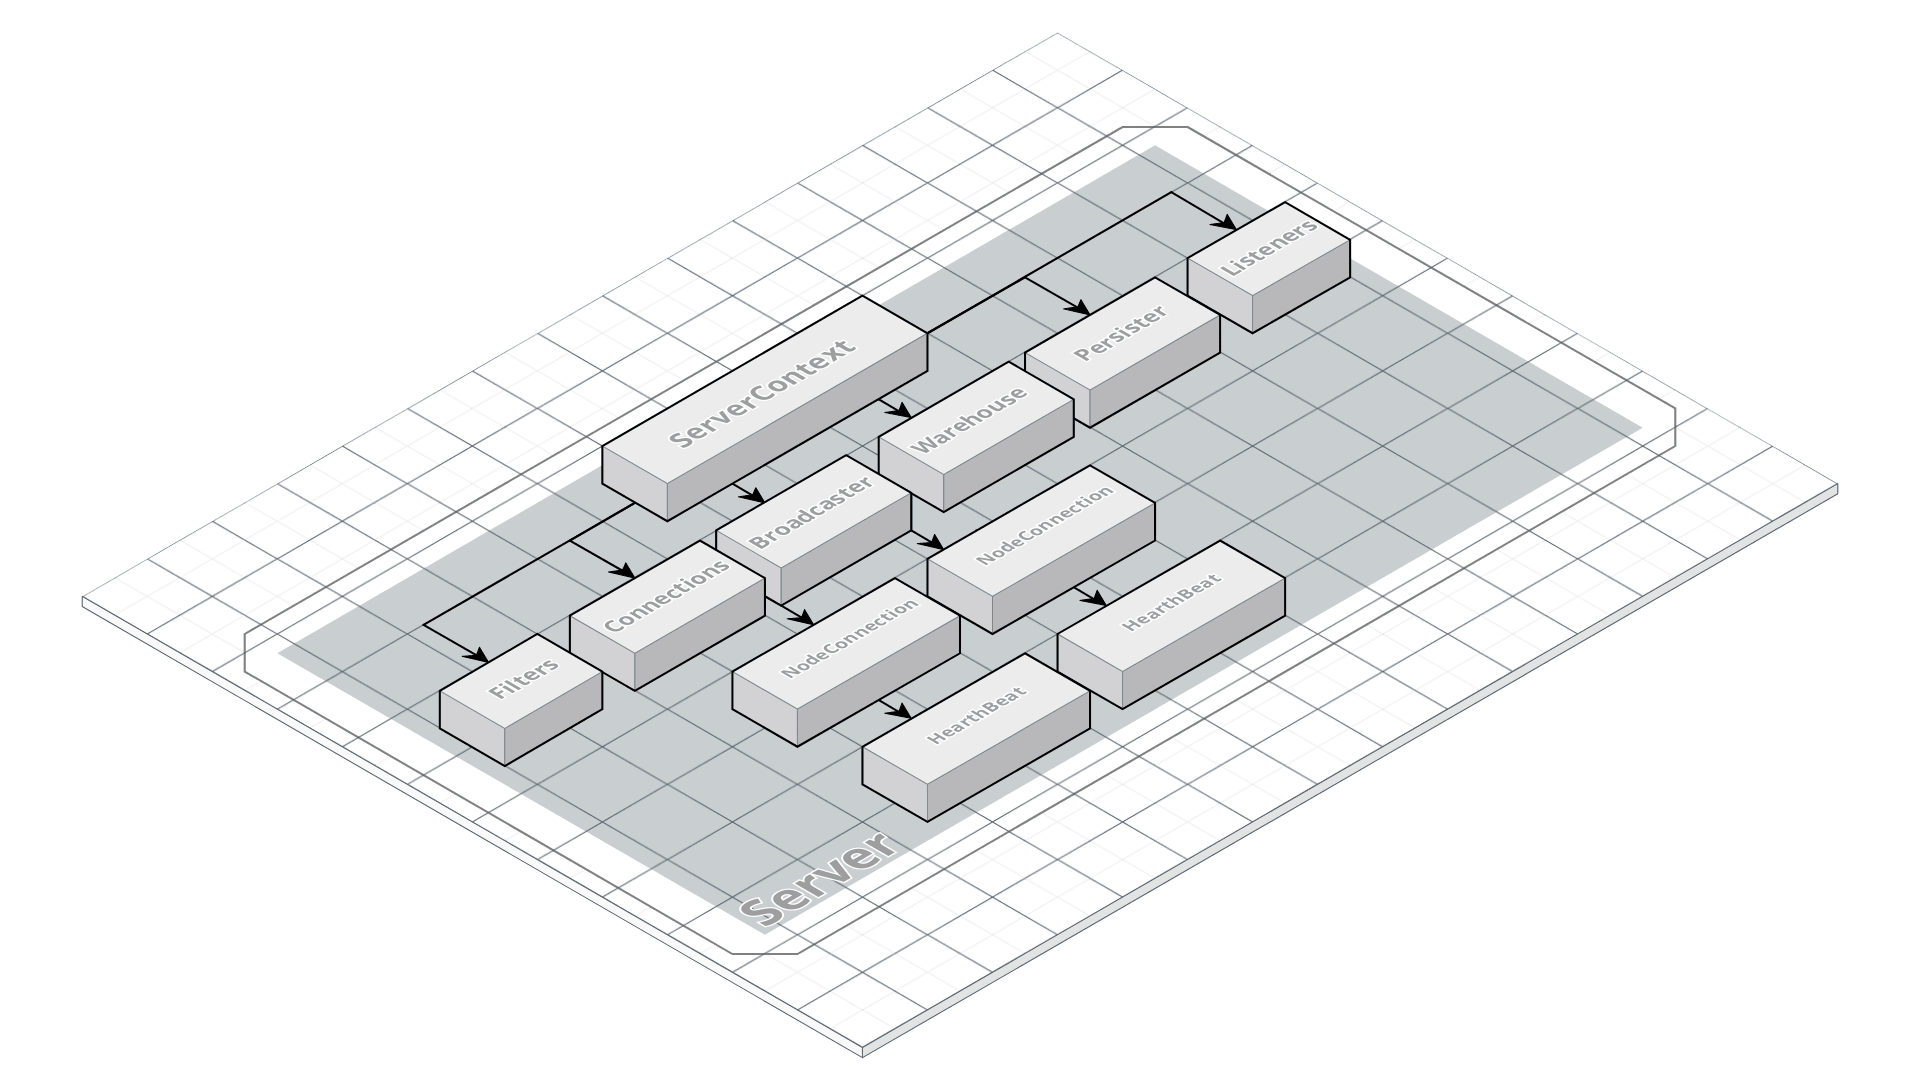
\includegraphics[width=\textwidth]{VS-Server-Context.png}
        
        \caption{Server-Context Aufbau}
        \label{}
    \end{figure}

    Sobald der ServerContext instanziiert wird, wird das Warehouse geladen. Zunächst wird versucht die Safe-Datei zu laden, scheitert das Laden wird das Warehouse leer instanziiert. Das Warehouse hält sämtliche Daten, die persistiert werden müssen (Messages, Chats, Users und gehandelte PacketIds). Der ServerContext erstellt außerdem den Persister. Der Persister ist ein Thread, der in regelmaßigen Abständen das Warehouse speichert (müsste in einer section schon beschrieben sein). Außerdem wird der Broadcaster erstellt, der die Verbindungen zu anderen Nodes hält und Broadcast-Packete an diese verteilt.
    Weitere Variablen sind isCloseRequested, die die "endlos" Schleifen aller Threads steuert und connections. Diese Liste hällt alle Connections zu Clients, die direkt zu dieser Node verbunden sind.

    Der Nodebroadcaster erstellt bei instanziierung je node einen eigenen Thread, der sich um das senden und das neu verbinden kümmert.
    Packete, die an eine Node gesendet werden soll werden sollen werden vom Broadcaster in die Queue geschrieben und die NodeConnection wird durch eine Semaphore aufgeweckt. Die NodeConnection versucht ein Packet zu senden. Scheitert das senden wird von einer Verbindungstrennung ausgegangen und die Verbindung wird neu verbunden.
    Zusätzlich besitzt die NodeConnection jeweils einen HeartBeat-Thread. Dieser Thread sendet regelmäßig ein Packet um zu testen, ob die Verbindung noch steht.

    Nachdem nun alle initialisierungs Vorgänge abgeschlossen sind, kann der ServerSocket erstellt werden und clients akzeptiert werden.
    Der Hauptserver-Thread ist dabei nur zuständig neue Verbindungen entgegenzunehmen. Für jede Verbindung wird ein ConnectionHandler-Thread erstellt, der sämtliche Nachrichten des Clients verarbeitet. Der Handler versucht dabei ein Packet vom Client zu lesen. Die Filter prüfen nun, ob das Packet gehandelt werden darf und wenn ja werden die passenden Handler mit dem Packet aufgerufen und die Filter aktualisieren sich.


    Filter:
    \begin{itemize}
        \item PacketIdFilter\\
            Der PacketId-Filter testet, ob ein Packet mit der Id bereits gesehen wurde. Nur wenn die Id neu ist darf das Packet gehandelt werden um recursive Broadcasts zu vermeiden. Bereits gesehene Packete werden im Warehouse mit gespeichert. Im seltenen Fall, dass die Node genau zwischen den Listenern und dem aktualisieren der Filter abstürzt kann es vorkommen, dass die gespeicherten packet ids nicht konsistenz zum Nutzdatenbestand sind. Hier könnte ein Transaktionsprotokoll implementiert werden. Da aber die Wahrscheinlichkeit dieses Fehlers äußerst gering ist wird hier darauf verzichtet.
    \end{itemize}
   


    Listener:
    \begin{itemize}
        \item BaseEntityBroadcastListener\\
            Der Listener behandelt BaseEntityBroadcastPackete, die ausgestrahlt werden, sobald ein neuer Nutzer, ein neuer Chat oder eine neue Nachricht erstellt wird. Die empfangene Entität wird in das Warehouse aufgenommen und weiter gesendet, falls es dieser Node neu war.
            Nachdem ein Chat erstellt wurde müssen die Clients, die an diesem Chat teilnehmen informiert werden. Da jede Node nur die direkt zu ihr verbundenen Clients kennt, muss jede Node prüfen ob sie einen teilnehmenden Client kennt und diesen informieren. Ähnliches gilt für neue Nutzer.
        \item CreateChatListener\\
            Dieser Listener erstellt Chats anhand von einem CreateChatPacket. Sofern das Packet von einem Nutzer kommt wird ein neuer Chat mit allen Teilnehmern und dem Absender erstellt und weiter verteilt.
        \item GetMessageListener\\
            Mithilfe eines GetMessagePackets können alle Nachrichten abgefragt werden, die in einem Chat gesendet wurden.
        \item KeyExchangeListener\\
            Dieser Listener leitet KeyExchangePackete von einem Client an andere Clients weiter (gegebenenfalls über andere Nodes).
        \item LoginListener\\
            Der LoginListener kümmert sich um die Authentifizierung eines Clients. Er prüft ob ein Nutzer besteht und falls ja wird das Passwort geprüft. Existiert noch kein Nutzer wird ein passender Nutzer erstellt. Anschließend wird der Client auf den neuesten Stand gebracht indem ein LoginSyncPacket an den Client gesendet wird. Dieses enthält die User id des aktuellen Nutzers, die anderen registrierten Nutzer und alle Chats, an dem der Client teilnimmt. Außerdem wird die Information der Connection gesetzt, zu welchem Client sie verbunden ist um ein gezieltes Senden zu ermöglichen (wie z.B. beim KeyExchange oder bei Messages).
        \item MessageListener\\
            Messages, die vom Client an einen Chat gesendet werden werden von diesem Listener bearbeitet. Der Listener kümmert sich dabei auch um die Verteilung der Nachrichten an alle anderen Chatteilnehmer.
        \item NodeSyncListener\\
            Wie in Fehlerbehandlung beschrieben müssen Nodes auf dem neuesten Stand gezogen werden, falls diese ausgefallen waren. Bei einem Reconnect wird ein NodeSyncPacket mit den aktuellen Informationen an die neu startende Node gesendet. Dieser Listener verarbeitet diese Packete indem er prüft ob eine Änderung vorliegt und wenn ja diese übernimmt und broadcastet. Theoretisch kann es sein, dass ein Nutzer sich anmeldet bevor die Node ihre Syncronisation abgeschlossen hat. Dieser Fehlerfall wird aber ignoriert, da die Syncronisationszeit und die Ausfallwahrscheinlichkeit einer Node als zu gering eingestuft wird.
    \end{itemize}


    Sollen hier andere Packete auch erkärt werden? Also Logout, GetMessageResponsePacket, NoOp, ...?
    
\end{document}